% % % Document Type
% http://www.biwako.shiga-u.ac.jp/sensei/kumazawa/tex/book.html
% http://ichiro-maruta.blogspot.jp/2013/03/latex.html
\RequirePackage[l2tabu, orthodox]{nag}
\documentclass[12pt, a4j, openany, uplatex, dvipdfmx]{jsarticle}

% % % Paper size
%\usepackage[top=1truein, bottom=1truein, left=1.5truein, right=1truein]{geometry} % 用紙サイズの設定のため

% % % Necessary
\usepackage{amssymb, amsmath, amsthm, latexsym} % For mathematics [Before hyperref]
\usepackage{empheq} % For mathematics
\usepackage[dvipdfmx,setpagesize=false]{hyperref} % For inserting hyperlink [Before graphicx]
\usepackage{pxjahyper} % https://texwiki.texjp.org/?hyperref
\usepackage[dvipdfmx]{graphicx} % For inserting figure
\usepackage[labelformat=simple]{subcaption} % For caption of figures and tables
%\renewcommand\thesubfigure{(\alph{subfigure})}
%\renewcommand\thesubtable{(\alph{subtable})}
\usepackage[usenames,dvipdfmx]{color} % For coloring
\usepackage[shortlabels]{enumitem} % For useful enumerate and itemize environment
\usepackage{comment} % For commenting multiline
\usepackage{cite} % For citing references [After hyperref]
\usepackage{url} % For inserting URL
\usepackage{acro} % For listing abbreviations and symbols
\usepackage{makeidx} % For making index

% % % Convenient for graph
\usepackage{tikz-cd} %load package after color.sty & soul.sty

% % % Convenient for tables and emphasis
\usepackage{tabularx} % For flexible table
\usepackage{multirow} % For combining multi rows for table
%\usepackage{colortbl} % For coloring table
\usepackage{longtable} % For long table across multiple pages
%\usepackage[normalem]{ulem} % For flexible underline etc.
%\usepackage{ascmac} % For framing multiline -> bxascmac に変更したほうがよい?

% % % 文書の見た目のためのパッケージ
\usepackage{setspace} % For single space or double space
\usepackage{afterpage} % For inseting newpage 
\usepackage{datetime} % For date style of title
\usepackage{fancyhdr} % For header and footer
% % tocloft を include すると目次の番号と文章が被る?
%\usepackage{tocloft} % 図目次、表目次の見た目を変えるため
\usepackage{pxrubrica} % For writing ruby

% % % Convenient for document of science and technology
\usepackage{numprint} % 数値の整形
\usepackage{siunitx} % For using SI units
\usepackage{listings} % For inserting programming code

% % % Option
\usepackage{docmute} % For compilation of divided files
\usepackage{bxcoloremoji} % For using emoji

% % % Reference for packages
% % empheq.sty
% http://muscle-keisuke.hatenablog.com/entry/2015/11/23/122725
% % geometry.styについて
% http://joker.hatenablog.com/entry/2012/07/09/153537
% % tocloft.styについて
% http://www.biwako.shiga-u.ac.jp/sensei/kumazawa/tex/tocloft.html
% http://tex.stackexchange.com/questions/20337/adding-word-table-before-each-entry-in-list-of-tables
% % makeidx.sty
% http://www.biwako.shiga-u.ac.jp/sensei/kumazawa/tex/makeidx.html
% % pxrubrica.sty
% https://qiita.com/zr_tex8r/items/42466cbcbeb670a3a2dc
% % %

% % % AMS-Theorem Environment
\theoremstyle{definition}

% 試験的に導入(定義を枠で囲むため).2005年だからパッケージとしては古いか?(もっといいのがあるかも)
% amsthm環境と競合するため,設定したあとで読み込む.
% https://ctan.org/tex-archive/macros/latex/contrib/thmbox
\usepackage[nocut, nounderline]{thmbox}
\thmboxoptions{titlestyle={\,(\textbf{#1})}}
\thmboxoptions{bodystyle=\upshape\noindent}
\newtheorem[S]{question}{問題}

% % % Config for hyperref
\hypersetup{ %
	breaklinks=true, %
	colorlinks=false, %
	urlcolor=blue, %
	urlbordercolor={0 1 1}}

% % % Define Command
\newcommand{\bm}[1]{\mbox{\boldmath $#1$}}
\newcommand{\dif}{\mathrm{d}}
\newcommand{\set}[1]{\left\{\,#1\,\right\}}
\newcommand{\im}{\operatorname{Im}}
\newcommand{\dom}{\operatorname{dom}}
\newcommand{\cod}{\operatorname{cod}}

% % % Re-define names

\begin{document}
	% % % Begin of Body
	% Chapterごとにファイルを分けて,それぞれをincludeする
	\section*{演習問題}
\begin{table}[!t]
	\begin{flushright}
		\begin{tabular}{rc}
			& \usdate\today \\
			学籍番号 & \\
			名前 & \\
		\end{tabular}
	\end{flushright}
\end{table}

別途,ノートかルーズリーフか白紙の計算用紙上に,計算過程も含めて,解いてください.

\begin{question}
	以下の多項式を因数分解せよ.
	\begin{enumerate}
		\item $x^2+6x+9$
		\item $x^2-2x-15$
		\item $x^3 - 3 x^2 - 13 x + 15$
		\item $x^3 - 3 x^2 - 10 x + 24$
	\end{enumerate}
\end{question}

\begin{question}
	以下の方程式,不等式を解け.
	\begin{enumerate}
		\item $x^2+6x+9 = 0$
		\item $x^2+6x+9 < 0$
		\item $x^2-2x-15 \geq 0$
		\item $x^3 - 3 x^2 - 13 x + 15 \leq 0$
	\end{enumerate}
\end{question}

\begin{question}
	以下の二次関数を平方完成し,グラフを図示せよ.また,それぞれの関数の像を求めよ.
	\begin{enumerate}
		\item $f(x) = x^2+6x+9$
		\item $g(x) = x^2-2x-15$
		\item $h(x) = -(x+2)(x-2)$
	\end{enumerate}
\end{question}

\begin{question}
	以下の代数関数のグラフを図示せよ.
	\begin{enumerate}
		\item $f(x) = 1/(x+2)$
		\item $g(x) = \sqrt{x+2}$
	\end{enumerate}
\end{question}

\vfill
\begin{figure}[!h]
	\centering
	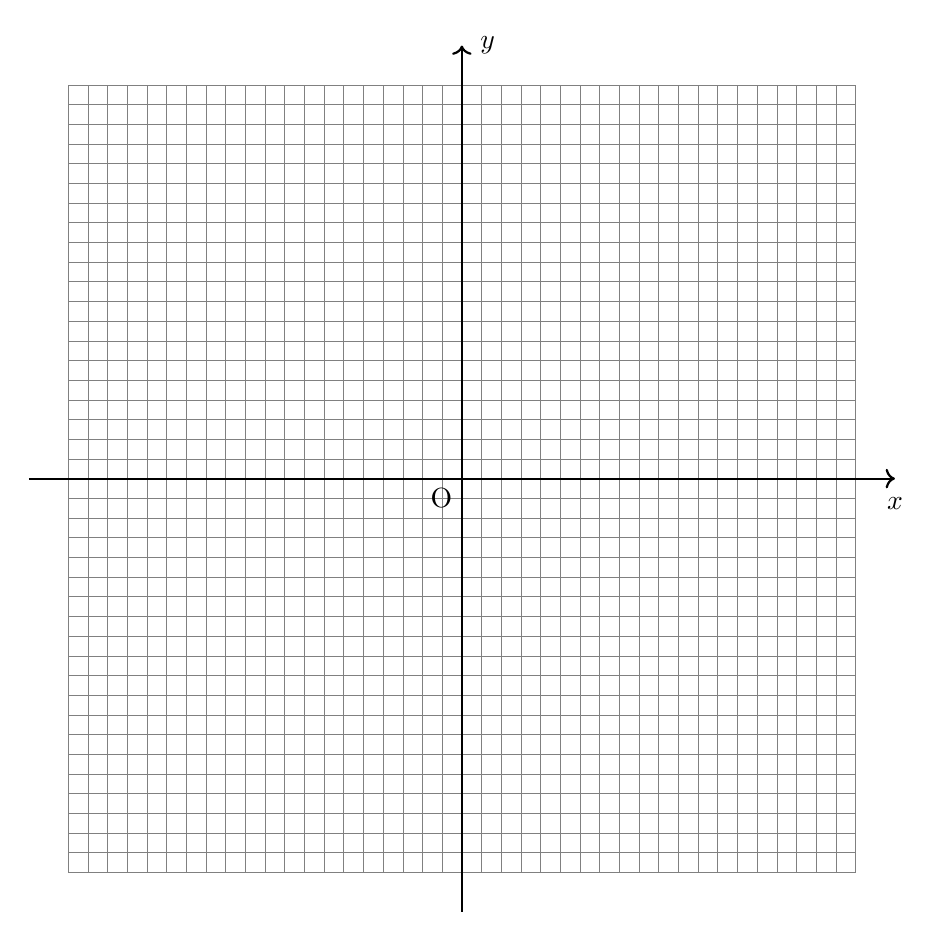
\begin{tikzpicture}
	\draw[help lines, step=0.25] (0,0) grid (10,10);
	\draw (5,5) node[below left]{O};
	\draw[thick, ->] (-0.5,5)--(10.5,5) node[below=3.0] {$x$};
	\draw[thick, ->] (5,-0.5)--(5,10.5) node[right=3.0] {$y$};
	\end{tikzpicture}
	\caption{$xy$平面}
	%\label{fig:quadraticFunction}
\end{figure}
\clearpage
	% % % End of Body
\end{document}
